%----------------------------------------------------------------
%	PACKAGES AND OTHER DOCUMENT CONFIGURATIONS
%----------------------------------------------------------------

\documentclass[landscape,a0paper,fontscale=0.285]{baposter} % Adjust the font scale/size here
\title{ETHz AFEA Cheat Sheet New}
\usepackage[brazilian]{babel}
\usepackage[utf8]{inputenc}

\usepackage{graphicx} % Required for including images
\graphicspath{{figures/}} % Directory in which figures are stored

\usepackage{xcolor}
\usepackage{colortbl}
\usepackage{tabu}
\usepackage[export]{adjustbox}

\usepackage{mathtools}
%\usepackage{amsmath} % For typesetting math
\usepackage{amssymb} % Adds new symbols to be used in math mode

\usepackage{booktabs} % Top and bottom rules for tables
\usepackage{enumitem} % Used to reduce itemize/enumerate spacing
\usepackage{palatino} % Use the Palatino font
\usepackage[font=small,labelfont=bf]{caption} % Required for specifying captions to tables and figures
\usepackage{multirow}
\usepackage{multicol} % Required for multiple columns
\setlength{\columnsep}{1.5em} % Slightly increase the space between columns
\setlength{\columnseprule}{0mm} % No horizontal rule between columns

\usepackage{tikz} % Required for flow chart
\usetikzlibrary{decorations.pathmorphing}
\usetikzlibrary{shapes,arrows} % Tikz libraries required for the flow chart in the template

\newcommand{\compresslist}{ % Define a command to reduce spacing within itemize/enumerate environments, this is used right after \begin{itemize} or \begin{enumerate}
\setlength{\itemsep}{1pt}
\setlength{\parskip}{0pt}
\setlength{\parsep}{0pt}
}

\definecolor{lightblue}{rgb}{0.145,0.6666,1} % Defines the color used for content box headers

\begin{document}

\begin{poster}
{
headerborder=closed, % Adds a border around the header of content boxes
colspacing=0.2em, % Column spacing
bgColorOne=white, % Background color for the gradient on the left side of the poster
bgColorTwo=white, % Background color for the gradient on the right side of the poster
borderColor=lightblue, % Border color
headerColorOne=lightblue, % Background color for the header in the content boxes (left side)
headerColorTwo=violet, % Background color for the header in the content boxes (right side)
headerFontColor=white, % Text color for the header text in the content boxes
boxColorOne=white, % Background color of the content boxes
textborder=roundedleft, % Format of the border around content boxes, can be: none, bars, coils, triangles, rectangle, rounded, roundedsmall, roundedright or faded
eyecatcher=true, % Set to false for ignoring the left logo in the title and move the title left
headerheight=0.03\textheight, % Height of the header
headershape=roundedright, % Specify the rounded corner in the content box headers, can be: rectangle, small-rounded, roundedright, roundedleft or rounded
headerfont=\Large\bf\textsc, % Large, bold and sans serif font in the headers of content boxes
%textfont={\setlength{\parindent}{1.5em}}, % Uncomment for paragraph indentation
linewidth=2pt % Width of the border lines around content boxes
}
%----------------------------------------------------------------
%	TÍTULO
%----------------------------------------------------------------
{\bf\textsc{ETHz APFEA Cheat Sheet}\vspace{0.0em}} % Poster title
{\textsc{E T H z \ \ \ \ A F E A \ \ \ \ \ C h e a t \ \ \ \ \ S h e e t \hspace{0pt}}}


%------------------------------------------------
% FEM
%------------------------------------------------
\headerbox{FEM \& Element}{name=fem,column=0,row=0}{\vspace{-0.3cm}
$$\vspace{-0.3cm}
Ku = f
$$
$K$: stiffness matrix 

$u$: displacement 

$f$: external force

\colorbox[HTML]{CCFFFF}{\makebox[\textwidth-2\fboxsep][l]{\bf - Stiffness Matrix}}
$$\vspace{-0.3cm}
K = \frac{EA}{l}\begin{bmatrix}
1 & -1 \\
-1 & 1
\end{bmatrix}
$$
$E$ : Young's Module

$A$ : section area

$l$ : characteristic length

\textbf{rotation}

\vspace{-1.4cm}
\begin{center}
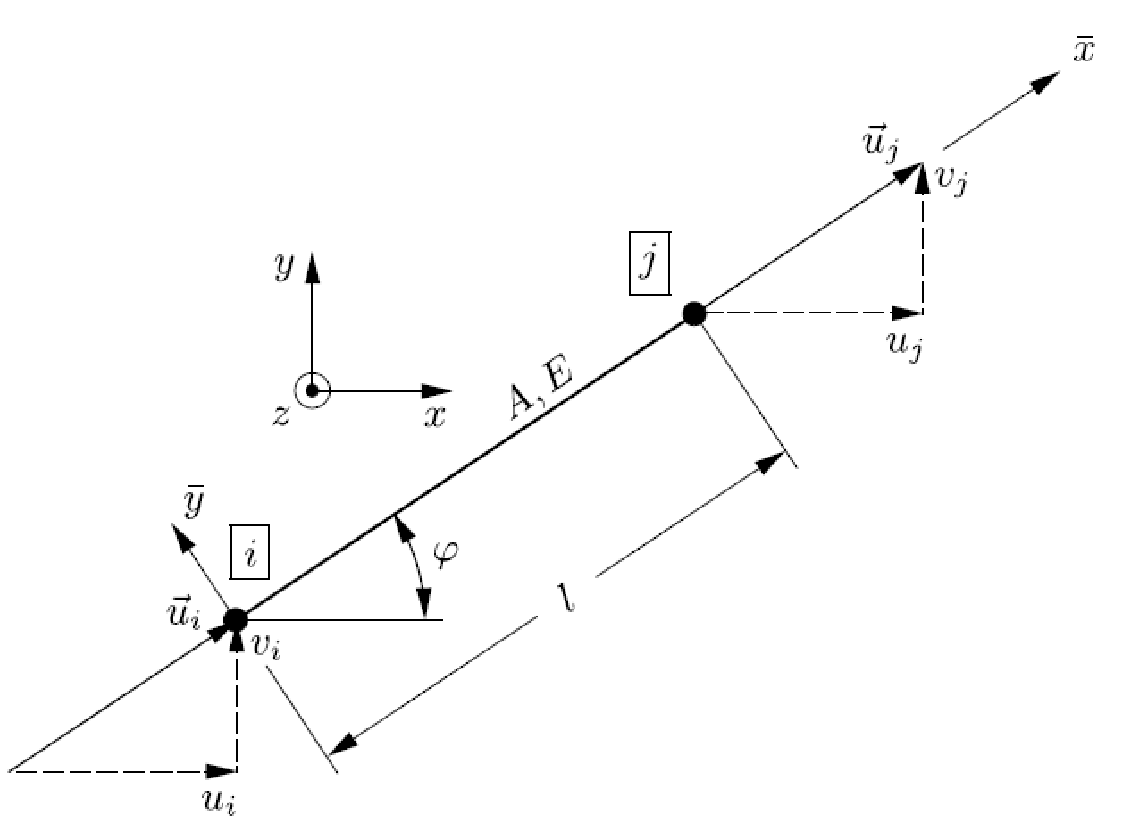
\includegraphics[width=0.7\textwidth]{figures/ETHz_AFEA_FEM_tranformation.png}
\end{center}
\vspace{-0.3cm}
$$\vspace{-0.3cm}
\begin{aligned}
&\hat K = 
\left[\begin{smallmatrix}
    cos\theta & sin\theta & 0 & 0 \\
    0 & 0 & cos\theta & sin\theta
\end{smallmatrix}\right]^\top
K 
\left[\begin{smallmatrix}
    cos\theta & sin\theta & 0 & 0 \\
    0 & 0 & cos\theta & sin\theta
\end{smallmatrix}\right]\\
 &= \frac{EA}{l}\left[\begin{smallmatrix}
     cos^2 & sin~cos & -cos^2 & -sin~cos\\
     sin~cos & sin^2 & -sin~cos & -sin^2 \\
     -cos^2 & -sin~cos & cos^2 & sin~cos \\
     -sin~cos & -sin^2 & sin~cos & sin^2
 \end{smallmatrix}\right]
 \end{aligned}
$$

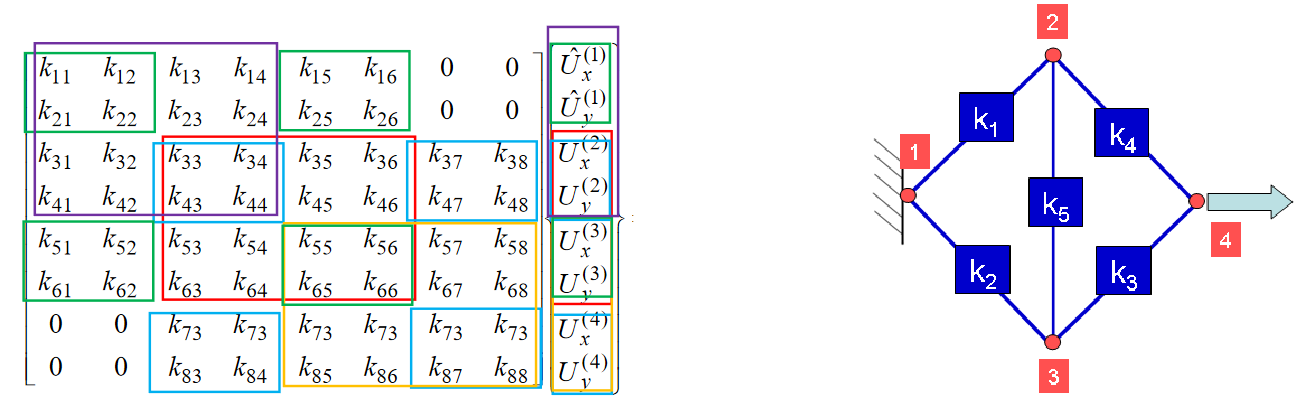
\includegraphics[width=\textwidth]{figures/ETHz_AFEA_FEM_stiffness.png}


\colorbox[HTML]{CCFFFF}{\makebox[\textwidth-2\fboxsep][l]{\bf - Continumm Elements}}

\textbf{Purpose} : Given the position of a point $r_j$ in local coordinate, compute the strain tensor $\varepsilon_{ii},\varepsilon_{i_1i_2}$ in global coordinate.
\vspace{-0.4cm}
$$\vspace{-0.4cm}
J_{ji} = \frac{\partial x_i(r_j)}{\partial r_j} = \frac{\partial \sum_k h^k(r_j)\hat x_i^k}{\partial r_j}
$$
\vspace{-0.4cm}
Interpolate(B matrix)
$$\vspace{-0.4cm}
\begin{aligned}
\varepsilon_{ii} &= \sum_k \frac{\partial h^k(r_j)}{\partial r_j}J_{ji}^{-1}\hat u_i^k
\\
2\varepsilon_{i_1i_2} &= \sum_k \frac{\partial h^k(r_j)}{\partial r_j}J_{j{i_1}}^{-1}\hat u_{i_1} + \frac{\partial h^k(r_j)}{\partial r_j}J_{j{i_2}}^{-1}\hat u_{i_2}
\end{aligned}
$$

$\hat u^k_i $: nodal $k$ displacement in global coordinate

$\hat x^k_i$ : nodal $k$ position in global coordinate

$x_i$: random point position in global coordinate

$r_j$: random point position in local coordinate 

$h^k(r_j)$ : nodal $k$ interpolate weight $\sum_k h^k(r_j) = 1$

$\varepsilon_{ii}$: diagnal of strain tensor $\boldsymbol \varepsilon$

$\varepsilon_{i_i,i_2}$ : triangle part of strain tensor  $\boldsymbol \varepsilon$


\resizebox{\textwidth}{!}{
\begin{tabular}{c|c|c|c}
    Element & Triangular & Tetrahedral & Hexahedral (Brick) \\
    Dimension & 2D & 3D & 3D\\
    Node & 3 & 4 & 6\\
\end{tabular}
}

}
%------------------------------------------------
% Element
%------------------------------------------------

\headerbox{Element}{name=element,column=1,row=0}{

\colorbox[HTML]{CCFFFF}{\makebox[\textwidth-2\fboxsep][l]{\bf - Continumm Elements}}

% \textbf{Purpose} : Given the position of a point $r_j$ in local coordinate, compute the strain tensor $\varepsilon_{ii},\varepsilon_{i_1i_2}$ in global coordinate.
% \vspace{-0.4cm}
% $$\vspace{-0.4cm}
% J_{ji} = \frac{\partial x_i(r_j)}{\partial r_j} = \frac{\partial \sum_k h^k(r_j)\hat x_i^k}{\partial r_j}
% $$
% \vspace{-0.4cm}
% Interpolate(B matrix)
% $$\vspace{-0.4cm}
% \begin{aligned}
% \varepsilon_{ii} &= \sum_k \frac{\partial h^k(r_j)}{\partial r_j}J_{ji}^{-1}\hat u_i^k
% \\
% 2\varepsilon_{i_1i_2} &= \sum_k \frac{\partial h^k(r_j)}{\partial r_j}J_{j{i_1}}^{-1}\hat u_{i_1} + \frac{\partial h^k(r_j)}{\partial r_j}J_{j{i_2}}^{-1}\hat u_{i_2}
% \end{aligned}
% $$

% $\hat u^k_i $: nodal $k$ displacement in global coordinate

% $\hat x^k_i$ : nodal $k$ position in global coordinate

% $x_i$: random point position in global coordinate

% $r_j$: random point position in local coordinate 

% $h^k(r_j)$ : nodal $k$ interpolate weight $\sum_k h^k(r_j) = 1$

% $\varepsilon_{ii}$: diagnal of strain tensor $\boldsymbol \varepsilon$

% $\varepsilon_{i_i,i_2}$ : triangle part of strain tensor  $\boldsymbol \varepsilon$


% \resizebox{\textwidth}{!}{
% \begin{tabular}{c|c|c|c}
%     Element & Triangular & Tetrahedral & Hexahedral (Brick) \\
%     Dimension & 2D & 3D & 3D\\
%     Node & 3 & 4 & 6\\
% \end{tabular}
% }

\textbf{Continuity}
\vspace{-0.3cm}
\begin{itemize}\compresslist
    \item C-0: element boundaries displacements
    \item C-1:Continuous 1st derivatives
\end{itemize}
\vspace{-0.3cm}

\textbf{Failed}

If the element is distorted or folded
there will be no 1-to-1 relationship
between natural and global
coordinates and the Jacobian will be singular

\textbf{Quadrilateral}
\vspace{-0.3cm}
$$\vspace{-0.3cm}
\hat u = \left[\begin{smallmatrix}
\hat u_x^1 & \hat u_y^1 & \hat u_x^2 & \hat u_y^2  &
\hat u_x^3 & \hat u_y^3 & \hat u_x^4 & \hat u_y^4
\end{smallmatrix}\right]^\top\\
$$
$$\vspace{-0.3cm}
\begin{aligned}
h^1 = 1/4(1-r_1)(1-r_2) \quad
h^2 = 1/4(1+r_1)(1-r_2) \\
h^3 = 1/4(1+r_1)(1+r_2) \quad 
h^4 = 1/4(1-r_1)(1+r_2)
\end{aligned}
$$
$$\vspace{-0.3cm}
\frac{\partial h^k}{\partial x_i} = \frac{\partial h^k}{\partial r_j} J^{-1}_{ji}
$$
$$\vspace{-0.3cm}
B = \left[\begin{smallmatrix}
\frac{\partial h^1}{\partial x_1} & 0 &
\frac{\partial h^2}{\partial x_1} & 0 &
\frac{\partial h^3}{\partial x_1} & 0 &
\frac{\partial h^4}{\partial x_1} & 0 \\
0 & \frac{\partial h^1}{\partial x_2} & 
0 & \frac{\partial h^2}{\partial x_2} & 
0 & \frac{\partial h^3}{\partial x_2} & 
0 & \frac{\partial h^4}{\partial x_2} \\
\frac{\partial h^1}{\partial x_1} & 
\frac{\partial h^1}{\partial x_2} & 
\frac{\partial h^2}{\partial x_1} &
\frac{\partial h^2}{\partial x_2} & 
\frac{\partial h^3}{\partial x_1} & 
\frac{\partial h^3}{\partial x_2} &
\frac{\partial h^4}{\partial x_1} & 
\frac{\partial h^4}{\partial x_2}
\end{smallmatrix}\right]
$$
$$
\left[\begin{smallmatrix}
    \epsilon_{11} & \epsilon_{22} & \epsilon_{12} + \epsilon_{21}
\end{smallmatrix}\right]^\top = B \hat u
$$

\colorbox[HTML]{CCFFFF}{\makebox[\textwidth-2\fboxsep][l]{\bf - Structual Elements}}

\textbf{Truss}:Stresses only in the axes direction
No bending resistance

\textbf{Beam}:With bending resistance

\textbf{Plate \& Shell}\vspace{-0.3cm}
\begin{itemize}\compresslist
    \item thickness is $0$
    \item perpendicular to the mid-surface
\end{itemize}
\vspace{-0.3cm}


\textbf{Kirchhof Shell}\vspace{-0.3cm}
 \begin{itemize}\compresslist
     \item  section perpendicular to the mid-surface
     \item infinite shear-stiffness:
for thin shell it's allowed,
for thick shell , deviations
to the real behavior occur 
    \item $C1$ continuity required
    \item Displacements and rotations are coupled
 \end{itemize}

\vspace{-0.3cm}

\textbf{Mindlin Shell}\vspace{-0.3cm}
\begin{itemize}\compresslist
    \item section may rotate, but still straight
    \item could be used for thick structures
    \item strong bending: Compression-strains go to infinity(aspect-ratio matters)
    \item $C0$ continuity required
    \item Displacements and rotations are independent of each other
\end{itemize}

\vspace{-0.3cm}


\colorbox[HTML]{CCFFFF}{\makebox[\textwidth-2\fboxsep][l]{\bf - Numerical Issues}}

\textbf{Volumetric Locking}
:
high order elements + reduced integration(reduce computation)

\textbf{Shear Locking}
:
Reduced integration avoid shear-locking effects,  may cause Hourglassing, controlled by adding artificial shear stiffness

\textbf{Hourglass Control}
:
avoid unphysical deformation of the structure (avoiding zero
energy modes)

}


%------------------------------------------------
% Continuum Mechanics
%------------------------------------------------

\headerbox{Continuum Mechanics}{name=results,column=2,span=1,row=0}{

\begin{center}
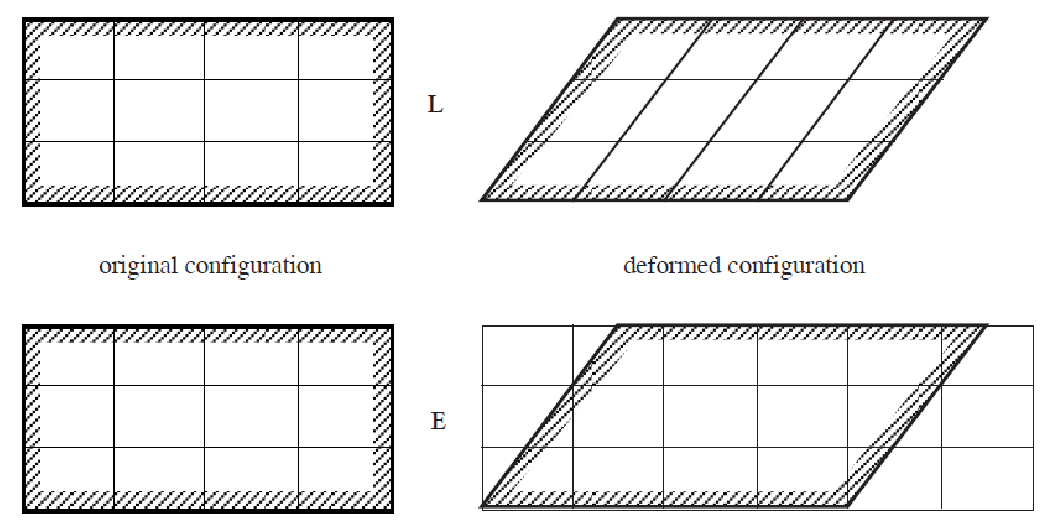
\includegraphics[width=0.6\textwidth]{figures/ETHz_AFEA_FEM_Continuum_configuration.png}

lagrangian(T) and eulerian(B) configuartion
\end{center}
\vspace{-0.4cm}
$$\vspace{-0.2cm}
x = X + u \quad dx = FdX
$$
$X$: is the origin position

$x$: transform position 

$u$: displacement

$F$: deformation gradient (not symmetric), $F=RU=VR$

\textbf{Right Cauchy Green Tensor}
:$C =F^\top F = U^T U$

\textbf{Left Cachy Green Tensor}
:$B = FF^\top = VV^\top$

\textbf{Engineering stress}:
$\sigma = \frac{F_t}{A_0}$

\textbf{Cauchy stress}:
$\sigma = \frac{F_t}{A_t}$

\colorbox[HTML]{CCFFFF}{\makebox[\textwidth-2\fboxsep][l]{\bf Green Langrange Strain Tensor}}\vspace{-0.3cm}
$$\vspace{-0.4cm}
E=\frac{1}{2}(F^\top F - I)
$$
$$\vspace{-0.2cm}
E_{ij} = \frac{1}{2}(u_{i,j} + u_{j,i} + u_{k,i}u_{k,j})
$$

\colorbox[HTML]{CCFFFF}{\makebox[\textwidth-2\fboxsep][l]{\bf first Piola-Kirchhoff stress}}\vspace{-0.3cm}
$$\vspace{-0.3cm}
P = J\sigma F^{-\top} \quad J=det(F)
$$

\begin{itemize}\compresslist
    \item not symmetric
    \item seldom used in
constitutive models
    \item axial stress same as Engineering stress
\end{itemize}

\colorbox[HTML]{CCFFFF}{\makebox[\textwidth-2\fboxsep][l]{\bf second Piola-Kirchhoff stress}}\vspace{-0.3cm}
$$\vspace{-0.3cm}
S = JF^{-1}\sigma F^{-\top} 
$$

\begin{itemize} \compresslist
    \item symmetric
    \item frequently used in
constitutive models
    \item not a clear physical meaning
    \item Corotational stress(objective)
    \item energy conjugate to Green
Lagrangian strain tensor($E$)
\end{itemize}


\colorbox[HTML]{CCFFFF}{\makebox[\textwidth-2\fboxsep][l]{\bf Spin tensor}}

$L$: velocity gradient, $L=\frac{dv}{dx}=\dot FF^{-1}$

$W$: asymmetric part of $L$, $W = \frac{1}{2}(L- L^\top)$, $W'=QWQ^\top+\dot QQ^{-1}$

objective: $\sigma' = Q\sigma Q^\top$, $Q$ is orthogonal

\textbf{Jaumann stress rate}\vspace{-0.3cm}
$$
\check \sigma = \dot \sigma + \sigma W - W\sigma
$$
take $\dot \sigma'$ and use $\dot Q=W'Q-QW$ and $\dot Q^\top = -Q^\top W' + QW$

\textbf{Truesdell stress rate}\vspace{-0.3cm}
$$
\check \sigma = \dot \sigma - L\sigma - \sigma L^\top + tr(L)\sigma
$$
}


%------------------------------------------------
% Continuum Mechanics
%------------------------------------------------

\headerbox{Elasto-Plastic}{name=results,column=3,span=1,row=0}{
$$
d\boldsymbol\varepsilon = d\boldsymbol\varepsilon^e + d\boldsymbol\varepsilon^p \quad d\boldsymbol\sigma = \mathbb C^e d\boldsymbol\varepsilon^e
$$
$\boldsymbol\varepsilon$: strain tensor, composed of elastic strain $\boldsymbol\varepsilon^e$ and plastic strain $\boldsymbol\varepsilon^p$

$\mathbb C^e$: 4-th order elasticity tensor

in uniaxial case, $\bar \sigma$ is equivalent stress

$\phi = \bar \sigma(\boldsymbol\sigma) - \sigma_y < 0$ elastic

$\phi = \bar \sigma(\boldsymbol\sigma) - \sigma_y = 0$ plastic

\textbf{Deviatoric Stress}:$\boldsymbol s = \boldsymbol\sigma - \frac{1}{3}tr(\boldsymbol\sigma)I$
\vspace{-0.3cm}
$$
J_1 = tr(\boldsymbol s) = 0\quad J_2 = \frac{1}{2}\boldsymbol s:\boldsymbol s \quad J_3 = det(\boldsymbol s)
$$

\colorbox[HTML]{CCFFFF}{\makebox[\textwidth-2\fboxsep][l]{\bf Von Mises stress }}

$$
\bar\sigma = \sqrt{3J_2} = \sqrt{\frac{1}{2}\sum_{i\neq j}[(\sigma_{ii}-\sigma_{jj})^2 + 6\sigma_{ij}^2]  }
$$

Equivalent Plastic Strain\vspace{-0.3cm}
$$\vspace{-0.3cm}
d\bar \varepsilon^p = \sqrt{\frac{2}{3}d\boldsymbol\varepsilon^p : d\boldsymbol\varepsilon^p}
$$

\colorbox[HTML]{CCFFFF}{\makebox[\textwidth-2\fboxsep][l]{\bf Normality Rule }}\vspace{-0.2cm}
$$\vspace{-0.6cm}
d\boldsymbol \varepsilon^p = d\bar \varepsilon^p\frac{\partial \phi}{\partial \boldsymbol\sigma}
$$
\begin{center}
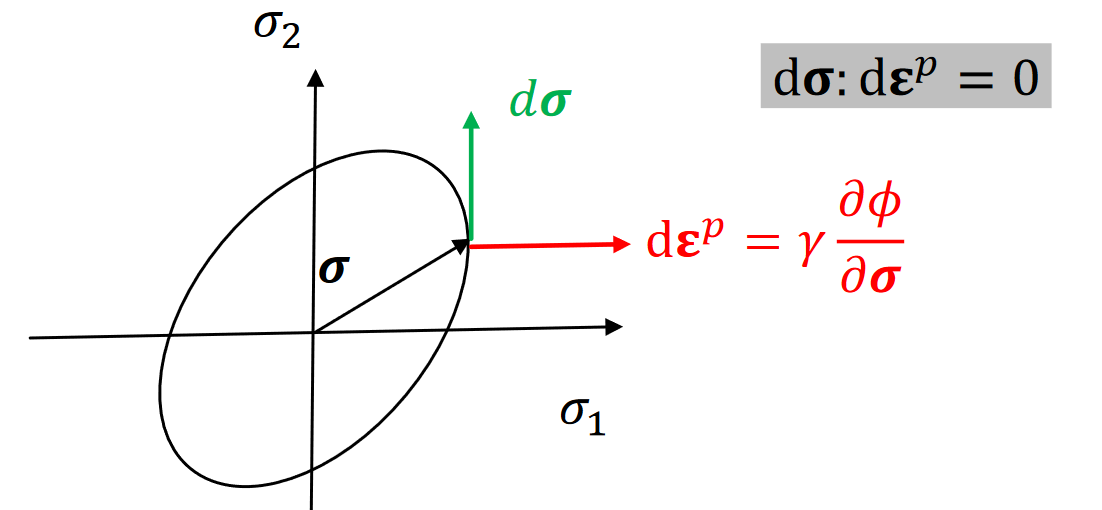
\includegraphics[width=0.7\textwidth]{figures/ETHz_AFEA_FEM_Elasto_Plastic_normal.png}
\end{center}


\colorbox[HTML]{CCFFFF}{\makebox[\textwidth-2\fboxsep][l]{\bf Hardening}}\vspace{-0.3cm}
$$\vspace{-0.3cm}
\phi = \bar\sigma(\boldsymbol\sigma) - \sigma_y(\bar \varepsilon^p) = 0
$$

\textbf{Consistency Condition}\vspace{-0.3cm}
$$\vspace{-0.3cm}
\frac{\partial \bar \sigma}{\partial \boldsymbol \sigma}d\boldsymbol \sigma - \frac{\partial \sigma_y}{\partial \bar\varepsilon^p}d\bar\varepsilon^p = 0
$$
\textbf{elastic-plastic masterial modulus}\vspace{-0.3cm}
$$\vspace{-0.3cm}
 \mathbb C^{ep} = \mathbb C^e(1-\frac{\frac{\partial \bar\sigma}{\partial \boldsymbol \sigma}:\mathbb C^e: \frac{\partial \bar \sigma}{\partial \boldsymbol \sigma}}{\frac{\partial \sigma_y}{\partial \bar \varepsilon^p}+\frac{\partial \bar\sigma}{\partial \boldsymbol \sigma}:\mathbb C^e: \frac{\partial \bar \sigma}{\partial \boldsymbol \sigma}})
$$

\textbf{return mapping algorithm}

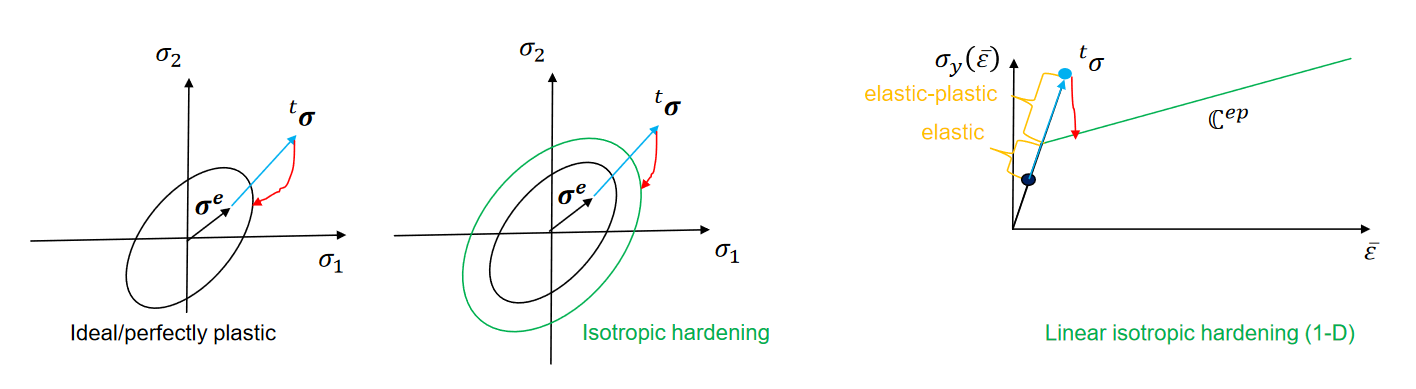
\includegraphics[width=\textwidth]{figures/ETHz_AFEA_FEM_Elasto_Plastic_return_mapping.png}


}




\end{poster}
\newpage

%%%%%%%%%%%%%%%%%%%%%%%%%%%%%%%%%%%%%%%%%%%%%%%%%%%%%%%%%%
%%%%%%%%%%%%%%%%%%    SEGUNDA PÁGINA    %%%%%%%%%%%%%%%%%%
%%%%%%%%%%%%%%%%%%%%%%%%%%%%%%%%%%%%%%%%%%%%%%%%%%%%%%%%%%

\begin{poster}
{
headerborder=closed, % Adds a border around the header of content boxes
colspacing=0.2em, % Column spacing
bgColorOne=white, % Background color for the gradient on the left side of the poster
bgColorTwo=white, % Background color for the gradient on the right side of the poster
borderColor=lightblue, % Border color
headerColorOne=lightblue, % Background color for the header in the content boxes (left side)
headerColorTwo=violet, % Background color for the header in the content boxes (right side)
headerFontColor=white, % Text color for the header text in the content boxes
boxColorOne=white, % Background color of the content boxes
textborder=roundedleft, % Format of the border around content boxes, can be: none, bars, coils, triangles, rectangle, rounded, roundedsmall, roundedright or faded
eyecatcher=true, % Set to false for ignoring the left logo in the title and move the title left
headerheight=0.03\textheight, % Height of the header
headershape=roundedright, % Specify the rounded corner in the content box headers, can be: rectangle, small-rounded, roundedright, roundedleft or rounded
headerfont=\Large\bf\textsc, % Large, bold and sans serif font in the headers of content boxes
%textfont={\setlength{\parindent}{1.5em}}, % Uncomment for paragraph indentation
linewidth=2pt % Width of the border lines around content boxes
}
%----------------------------------------------------------------
%	TÍTULO
%----------------------------------------------------------------

{\bf\textsc{E T H z \ \ \ \ A F E A \ \ \ \ \ C h e a t \ \ \ \ \ S h e e t }\vspace{0.0em}} % Poster title
{}

%----------------------------------------------------------------
%	Hyper Elastic
%----------------------------------------------------------------
\headerbox{Hyper-Elastic}{name=method,column=0}{
incompressible material\vspace{-0.3cm}
$$\vspace{-0.2cm}
\begin{aligned}
\boldsymbol\varepsilon &= \boldsymbol \varepsilon' + \frac{1}{3}\varepsilon_V \boldsymbol I\\
\boldsymbol \sigma &= \kappa \varepsilon_V \boldsymbol I + 2 G \boldsymbol\varepsilon' = -p\boldsymbol I + 2G\boldsymbol\varepsilon'
\end{aligned}
$$
$\boldsymbol\varepsilon'$: devitoric strain tensor

$\varepsilon_V$:  volumetric strain

$\kappa$: Bulk modulus, $\kappa = \frac{E}{3(1-2\nu)}$

$G$: Shear modulus, $G=\frac{E}{1+\nu}$

$p$: pressure, $p = -\frac{1}{3}Tr(\boldsymbol\sigma) = -\kappa \varepsilon_V$

$$
\left[\begin{smallmatrix}
    K_{uu} & K_{up}\\
    K_{pu} & K_{pp}
\end{smallmatrix}\right]
\left[\begin{smallmatrix}
    \hat u \\ \hat p
\end{smallmatrix}\right] = 
\left[\begin{smallmatrix}
    f^{ext}\\0
\end{smallmatrix}\right]
$$

if material total incompressible $\kappa\rightarrow \infty, K_{pp}\rightarrow 0 $

\colorbox[HTML]{CCFFFF}{\makebox[\textwidth-2\fboxsep][l]{\bf Mixed Formulations}}
\vspace{-0.5cm}
\begin{center}
% 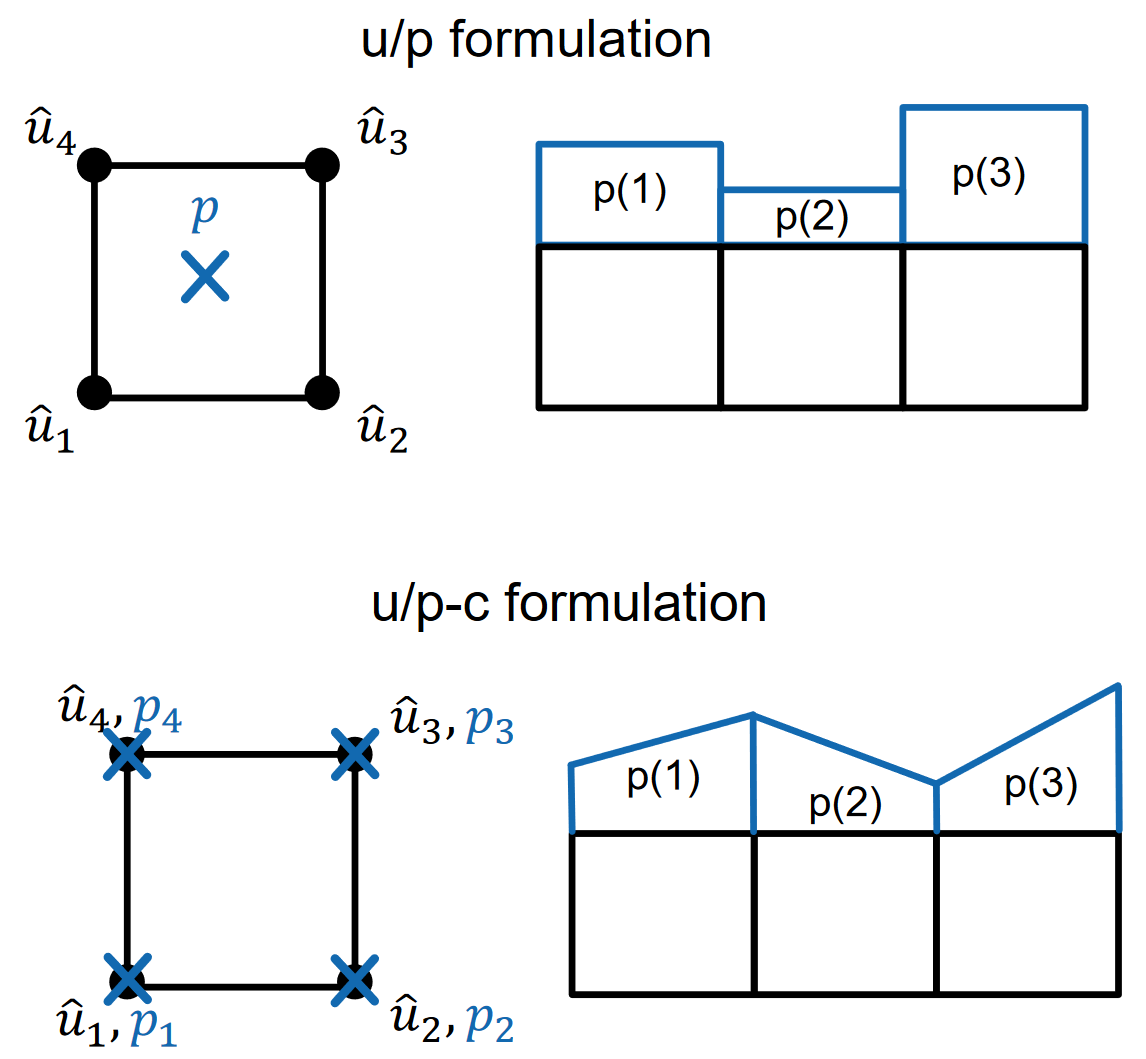
\includegraphics[width=0.7\textwidth]{figures/ETHz_AFEA_FEM_Hyper_Elastic_mixed_formulation.png}
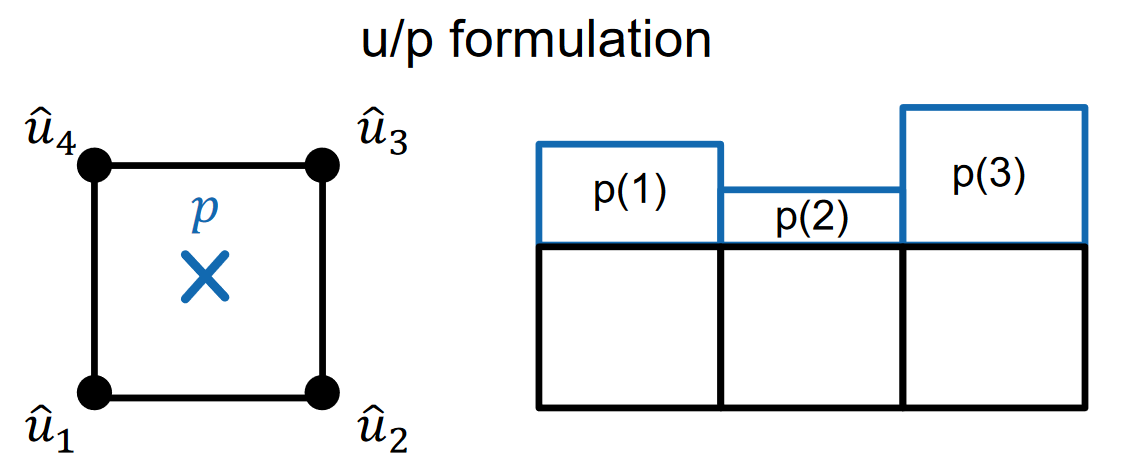
\includegraphics[width=0.6\textwidth, trim={0 0.2cm 0 0.2cm},clip]{figures/ETHz_AFEA_FEM_Hyper_Elastic_mixed_formulation_a.png}
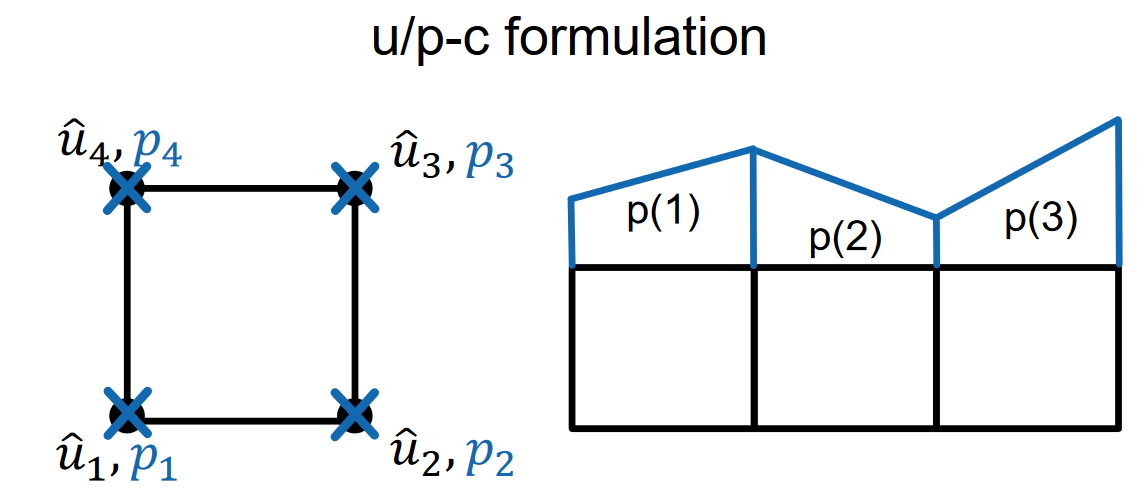
\includegraphics[width=0.6\textwidth, trim={0 0.2cm 0 0.2cm},clip]{figures/ETHz_AFEA_FEM_Hyper_Elastic_mixed_formulation_b.png}
\end{center}
\vspace{-0.2cm}
\textbf{Right Cauchy stress tensor} : $C = F^\top F = diag(\lambda_i^2)$\vspace{-0.3cm}

$$\vspace{-0.2cm}
\begin{aligned}
I_1 &= Tr(C) = \sum_i \lambda_i^2 \\
I_2 &= \frac{1}{2}(Tr(C)^2 - Tr(C^2)) \\
I_3 &= det(C)
\end{aligned}
$$


\colorbox[HTML]{CCFFFF}{\makebox[\textwidth-2\fboxsep][l]{\bf Neo-Hook Model}}\vspace{-0.3cm}
$$\vspace{-0.3cm}
W = \frac{1}{2}G(I_1 - 3)
$$
\begin{itemize}\compresslist
    \item tensile test same as first Piola-Kirchhof stress
    \item accurate only for small strain
    \item only one parameter $G$
\end{itemize}

\colorbox[HTML]{CCFFFF}{\makebox[\textwidth-2\fboxsep][l]{\bf Mooney Model}}\vspace{-0.3cm}
$$\vspace{-0.3cm}
W=C_1(I_1 - 3) + C_2\left(\frac{1}{\lambda_1^2} +\frac{1}{\lambda_2^2} + \frac{1}{\lambda_3^2}-3\right)
$$
assumption
\begin{itemize}\compresslist
    \item incompressible and isotropic
    \item obeys Hooke’s law under simple shear
\end{itemize}

\colorbox[HTML]{CCFFFF}{\makebox[\textwidth-2\fboxsep][l]{\bf Other Model}}
\textbf{Mooney Rivlin Model}:$W = C_1(I_1-3) + C_2(I_2-3)$

\textbf{Ogden Model}:$W = \sum_{k=1}^N\frac{\mu_k}{\alpha_k}(\lambda_1^{\alpha_k} + \lambda_2^{\alpha_k} + \lambda_3^{\alpha_k - 3})$
}


%----------------------------------------------------------------
%	Quasi-Static Implicit / Dynamic Explicit FEM
%----------------------------------------------------------------
\headerbox{Implicit Quasi-Static FEM}{name=results2,column=1}{
$$\vspace{-0.3cm}
K(u)\Delta u = \Delta F
$$
\colorbox[HTML]{CCFFFF}{\makebox[\textwidth-2\fboxsep][l]{\bf Full Newton-Raphson }}\vspace{-0.3cm}


% \underline{\textbf{}}\vspace{-0.3cm}
$$\vspace{-0.3cm}
K^i \Delta u^{i+1} = \Delta f^{i}
$$
quadratic convergence rate.

% \textbf{Pros}:Fast (even quadratic) convergence rate.

% \textbf{Cons}:stiffness matrix reformed iteration (costly)


\underline{\textbf{Modified Newton-Raphson}}\vspace{-0.2cm}
$$\vspace{-0.3cm}
K^0 \Delta u^{i+1} = \Delta f^{i}
$$

% \textbf{Pros}:Stiffness matrix only formed  once

% \textbf{Cons}:more iterations needed

\underline{\textbf{Quasi Newton-Methods}}

secant approximation

BFGS method
% \vspace{-0.2cm}
% $$\vspace{-0.2cm}
% ^{t+\Delta t}K^{i+1}(^{t+\Delta t}\Delta u^{i+1} - ^{t+\Delta t}\Delta u^i) = f^{i+1}_{ext} - f^i_{ext}
% $$


\textbf{Convergence Criteria}

convergence check for each iteration\vspace{-0.2cm}
\begin{itemize}\compresslist
    \item Displacement:$\frac{\Vert \Delta u^{i+1}\Vert_2}{\Vert ^{t+\Delta t}u\Vert_2} \le TOL_{dsp}$
    \item Residual:$\frac{\Vert ^{t+\Delta t}f_{ext} - ^{t+\Delta t}f_{int}\Vert_2}{\Vert ^{t+\Delta t}f_{ext} - ^{t}f_{int} \Vert} \le TOL_{res}$
\end{itemize}


\colorbox[HTML]{CCFFFF}{\makebox[\textwidth-2\fboxsep][l]{\bf Linear  System Solver }}\vspace{-0.3cm}

% \underline{\textbf{Linear  System Solver}}\vspace{-0.2cm}
\begin{center}
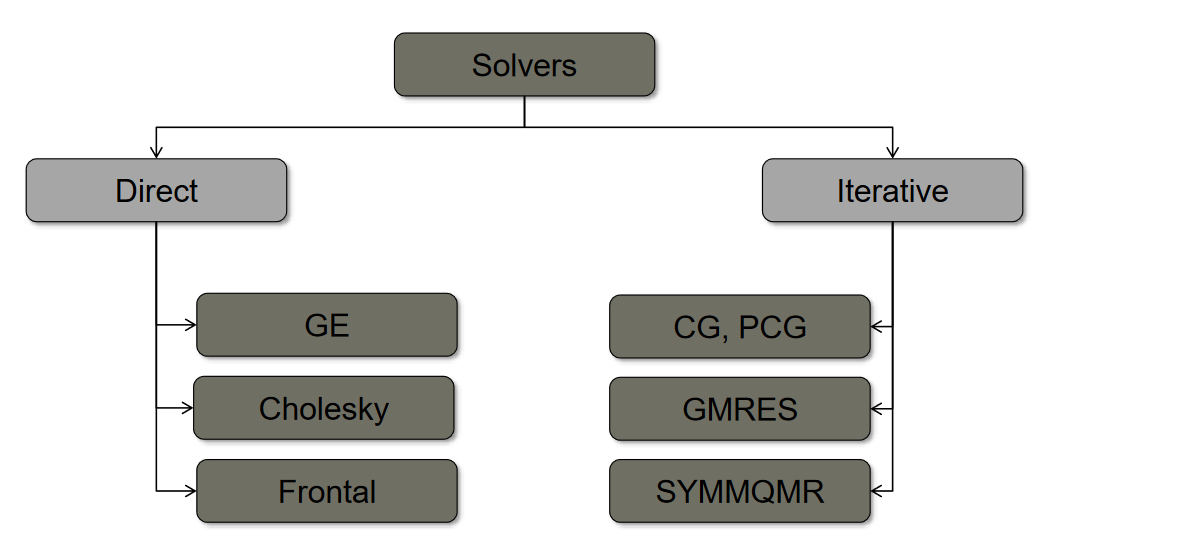
\includegraphics[width=\textwidth, trim={0 0.2cm 0.5cm 1cm},clip]{figures/ETHz_AFEA_FEM_Implicit_Solution_iteration.png}
\end{center}\vspace{-0.3cm}

CG solver should be definite

% \colorbox[HTML]{CCFFFF}{\makebox[\textwidth-2\fboxsep][l]{\bf Solution of Linear Systems of Equations}}\vspace{-0.3cm}
% $$\vspace{-0.3cm}
% K_{n\times n }u_{n\times 1} = f_{n\times 1}
% $$

% \underline{\textbf{Direct Solvers}}

% based on Gauss – Jordan elimination algorithm

% Pros\vspace{-0.2cm}
% \begin{itemize}\compresslist
%     \item Predictable number of operations and accuracy
%     \item Fast for small to midsize systems
% \end{itemize}

% \vspace{-0.2cm}
% Cons\vspace{-0.2cm}
% \begin{itemize}\compresslist
%     \item Large storage requirements
%     \item Slow performance for large systems
%     \item Hard to parallelize
% \end{itemize}
% \vspace{-0.2cm}

% \underline{\textbf{Iterative Methods}}
% conjugated-gradient(cg) solver

% Pros\vspace{-0.2cm}
% \begin{itemize}\compresslist
%     \item Much smaller storage requirements than direct solvers
%     \item Usually only few matrix times vector operations needed per iteration
%     \item Solution found up to desired accuracy
%     \item Usually easy to parallelize
% \end{itemize}

% \vspace{-0.2cm}
% Cons\vspace{-0.2cm}
% \begin{itemize}\compresslist
%     \item Convergence is not necessarily guaranteedv
%     \item Badly conditioned systems may show extremely slow convergence
% \end{itemize}
% \vspace{-0.2cm}
\underline{\textbf{Direct Solver}}

based on Gauss – Jordan elimination algorithm

Advantage\vspace{-0.2cm}
\begin{itemize}\compresslist
    \item  predicable number of operations and acc
    \item fast for small to midsize systems
\end{itemize}
\vspace{-0.2cm}
Disadvantage\vspace{-0.2cm}
\begin{itemize}\compresslist
    \item large storage requirements
    \item slow performance for large system
    \item hard to parallel
\end{itemize}
\vspace{-0.2cm}

\underline{\textbf{Iterative Solver}}

Advantage\vspace{-0.2cm}
\begin{itemize}\compresslist
    \item smaller storage
    \item few operations
    \item found up to desired accuracy
    \item easy to parallel
\end{itemize}
\vspace{-0.2cm}

Disadvantage\vspace{-0.2cm}
\begin{itemize}\compresslist
    \item Convergence not gauranteed
    \item badly conditioned system slow convergence
\end{itemize}\vspace{-0.2cm}


\textbf{Sparse Storage}\vspace{-0.2cm}
\begin{itemize}\compresslist
    \item Banded Storage: along diagonal
    \item Skyline Storage: along column near diagonal
    \item CSR and CSC (no $0$ value)
\end{itemize}

% \colorbox[HTML]{CCFFFF}{\makebox[\textwidth-2\fboxsep][l]{\bf Explicit Dynamic FEM}}\vspace{-0.2cm}
% $$\vspace{-0.2cm}
% M\ddot u + C\dot u + Ku = F
% $$
% $$\vspace{-0.2cm}
% u^{t+\Delta t} = \hat M^{-1}\hat f
% $$
% $\hat M$  : effective mass(diagonal)

% $\hat f$ : effective load
% \vspace{-0.4cm}
% $$\vspace{-0.2cm}
% \Delta t_{crit} = \frac{L_{char}}{c}
% $$
% $$\vspace{-0.2cm}
% T_{tot}^{CPU} \propto \frac{t_{process}}{\Delta t_{critic}}
% $$
% explicit method not suitable for \vspace{-0.2cm}
% \begin{itemize}\compresslist
%     \item spring back analysis
%     \item incompressible material
%     \item small plasitic zone but large deformation
% \end{itemize}
}


%----------------------------------------------------------------
%	Quasi-Static Implicit / Dynamic Explicit FEM
%----------------------------------------------------------------
\headerbox{Dynamic  FEM}{name=results2,column=2}{

time dependent problem (time integration)
\begin{itemize}\compresslist
    \item implicit dynamic FEM
    \item explicit dynamic FEM
\end{itemize}
\vspace{-0.3cm}
$$\vspace{-0.2cm}
M\ddot u + C\dot u + Ku = F
$$

\colorbox[HTML]{CCFFFF}{\makebox[\textwidth-2\fboxsep][l]{\bf Explicit Dynamic FEM}}\vspace{-0.2cm}

$$\vspace{-0.2cm}
\begin{aligned}
u^{t+\Delta t} &= \hat M^{-1}\hat f\\
\ddot u &= \frac{u^{t+\Delta t} - 2u^t + u^{t-\Delta t}}{\Delta t^2}\\
\dot u &= \frac{u^{t+\Delta t} - u^{t-\Delta t}}{2\Delta t}
\end{aligned}
$$
$\hat M$  : effective mass(diagonal)

$\hat f$ : effective load
\vspace{-0.4cm}
$$\vspace{-0.2cm}
\Delta t_{crit} = \frac{L_{char}}{c}
$$
$$
T_{tot}^{CPU} \propto \frac{t_{process}}{\Delta t_{critic}}
$$
init:$u^{-\Delta t} = u^0 -\dot u^0 \Delta t + \ddot u^0 \frac{\Delta t^2}{2}$

accelerate computation
\begin{itemize}\compresslist
    \item \textbf{time scaling}: increase velocity
    \item \textbf{mass scaling}: increase density
\end{itemize}

\resizebox{\textwidth}{1cm}{
\begin{tabular}{c|c|c}
     Bar &  $c=\sqrt{\frac{E}{\rho}}$ & $l_{char} = L$\\
     \multirow{2}*{Shell}& \multirow{2}*{$c=\sqrt{\frac{E}{(1-\nu^2)\rho}}$} & quadraliteral $l_{char} = \frac{A}{min(l_{max}, d_{max})}$\\
     & & triangluera $l_{char} = frac{A}{h_{min}}$\\
     \multirow{2}*{3D Solid}& \multirow{2}*{$c=\sqrt{\frac{E(1-\nu)}{(1+\nu)(1-2\nu)\rho}}$} & Hexadral $l_{char} = \frac{V}{A_{max}}$\\
     && Tetrahedral $l_{char} = h_{min}$
\end{tabular}
}

% 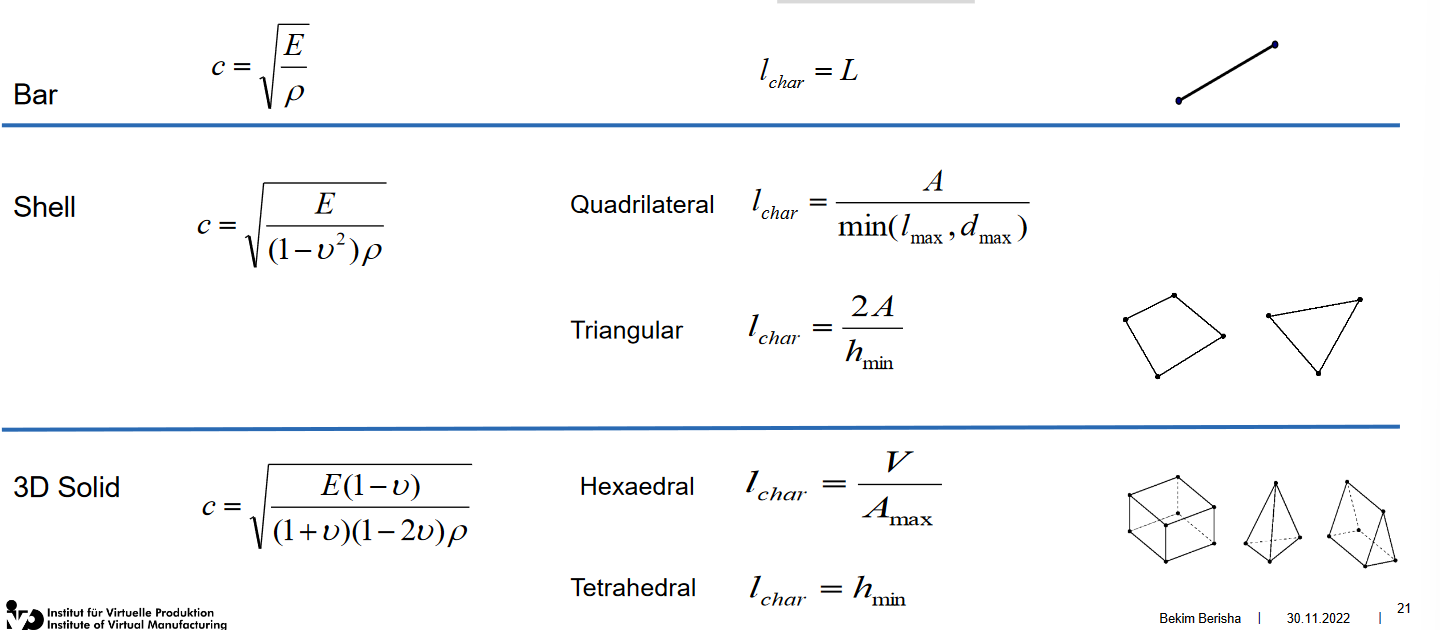
\includegraphics[width=\textwidth]{figures/ETHz_AFEA_FEM_Dynamic_critc_step.png}

explicit method not suitable for \vspace{-0.2cm}
\begin{itemize}\compresslist
    \item slow processed
    \item spring back analysis
    \item incompressible material
    \item small plastic zone but large deformation
\end{itemize}

\resizebox{\textwidth}{1.7cm}{
\begin{tabular}{c|c|c}
&QS Implicit& QS Explicit\\
Equilibrium & $\checkmark$ & $\times$ \\
Time step & arbitrary & $\Delta t < \Delta t_{char}$ \\ 
Convergence & stable & conditionally stable\\
Boundary & RB suppressed & free\\
Contact & iterated & not iterated \\
Rezoning & $t_{fine}=t_{course}$ & $\Delta t_{critic}^{new} = \frac{1}{2}\Delta t_{cirtic}^{old}$ \\ 
Stiffness matrix & evaluated & not computed  \\
Parallelization & complex & easy \\
\end{tabular}
}

}



%----------------------------------------------------------------
%	Instability and Boundary and Thermo coupled
%----------------------------------------------------------------
\headerbox{Instability \& Boundary \& Coupled}{name=conclusion,column=3,span=1,row=0}{
\colorbox[HTML]{CCFFFF}{\makebox[\textwidth-2\fboxsep][l]{\bf Instablility}}
\begin{center}
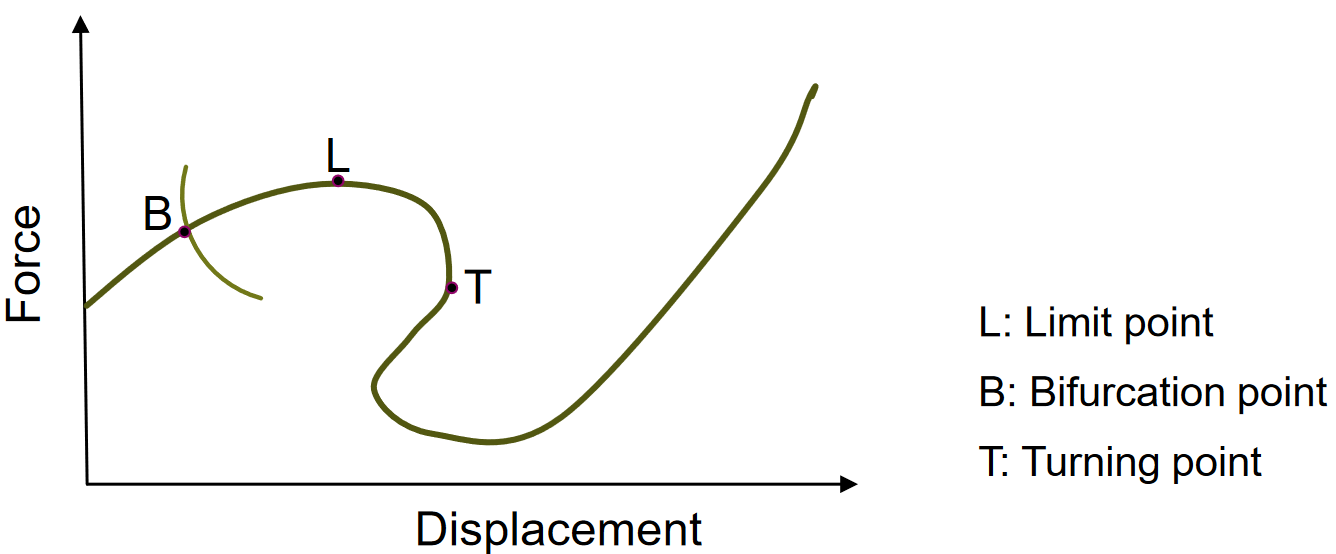
\includegraphics[width=0.8\textwidth]{figures/ETHz_AFEA_FEM_invalid_force_displacement.png}
\end{center}
\underline{\textbf{Arc-Length method}}
$$
\boldsymbol r(\boldsymbol u, \lambda) := \hat f^{int}(\boldsymbol u(t)) - \lambda(t)\boldsymbol f_0^{ext} = 0
$$
$$
g(\boldsymbol u(t),\lambda(t)):=\sqrt{\Vert \dot{\boldsymbol u} \Vert^2+\vert \dot \lambda \vert^2} - \dot s = 0
$$
$\dot s$ is the chosen value

$n+1$ unkowns

\colorbox[HTML]{CCFFFF}{\makebox[\textwidth-2\fboxsep][l]{\bf Contact}}

\textbf{Lagrange Multiplier Method}
$$
\begin{bmatrix}
K& e_i \\
e_i^\top & 0
\end{bmatrix}
\begin{bmatrix}
U\\ \lambda 
\end{bmatrix}
= \begin{bmatrix}
R\\ U_i*
\end{bmatrix}
$$
loss band structure of $K$

$\lambda$ is additional variable

\textbf{Penalty method}
$$
(K+\alpha Z^\top Z)U = R+\alpha Z^\top V
$$
boundary condition : $ZU = V$

$U$ is nodal displacement


\colorbox[HTML]{CCFFFF}{\makebox[\textwidth-2\fboxsep][l]{\bf Thermo coupled}}

\begin{center}
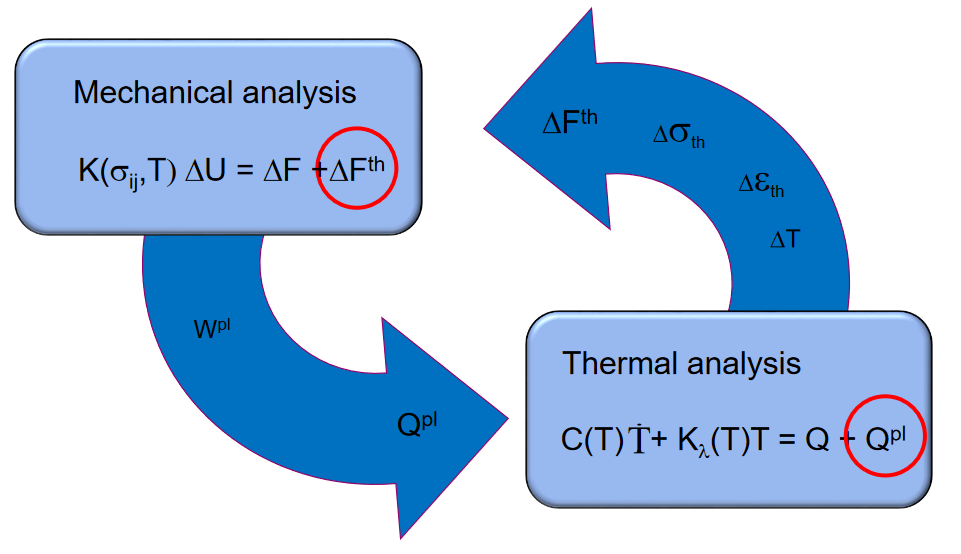
\includegraphics[width=0.8\textwidth]{figures/ETHz_AFEA_FEM_Thermo_coupled.png}
\end{center}

Heating source
\begin{itemize}\compresslist
    \item plastic work
    \item friction
    \item heat transfer
\end{itemize}

}

% %----------------------------------------------------------------
% %	Coupled Problem
% %----------------------------------------------------------------
% \headerbox{Coupled Problem}{name=conclusion,column=3,span=1,row=0}{
% }


%----------------------------------------------------------------
%	REFERENCES  {name=objectives,column=0,row=0}
%----------------------------------------------------------------
%\headerbox{bb}{name=references,column=1,row=0}{}
%----------------------------------------------------------------
%	FUTURE RESEARCH
%----------------------------------------------------------------
%\headerbox{aa}{name=futureresearch,column=1,row=0}{}
%----------------------------------------------------------------
%	CONTACT INFORMATION
%----------------------------------------------------------------
%\headerbox{Contact Information}{name=contact,column=2,span=2,row=0}{}
%----------------------------------------------------------------
\end{poster}
\end{document}